\pagenumbering{arabic} %從這頁開始用數字頁碼

\chapter{Introduction} 
%cite放在./Part/Reference,如果Thesis.tex第一次看到這個位置,他不知道要到下面去找,要編譯兩次才會出現引用編號。


%==================== Higgs ====================%
\section{The Discovery of the Higgs Boson}
The Higgs boson is discovered ..

\begin{figure}[!h]
	\graphicspath{ {./Figures/} }
	\centering
	\begin{minipage}[h]{0.45\textwidth}
		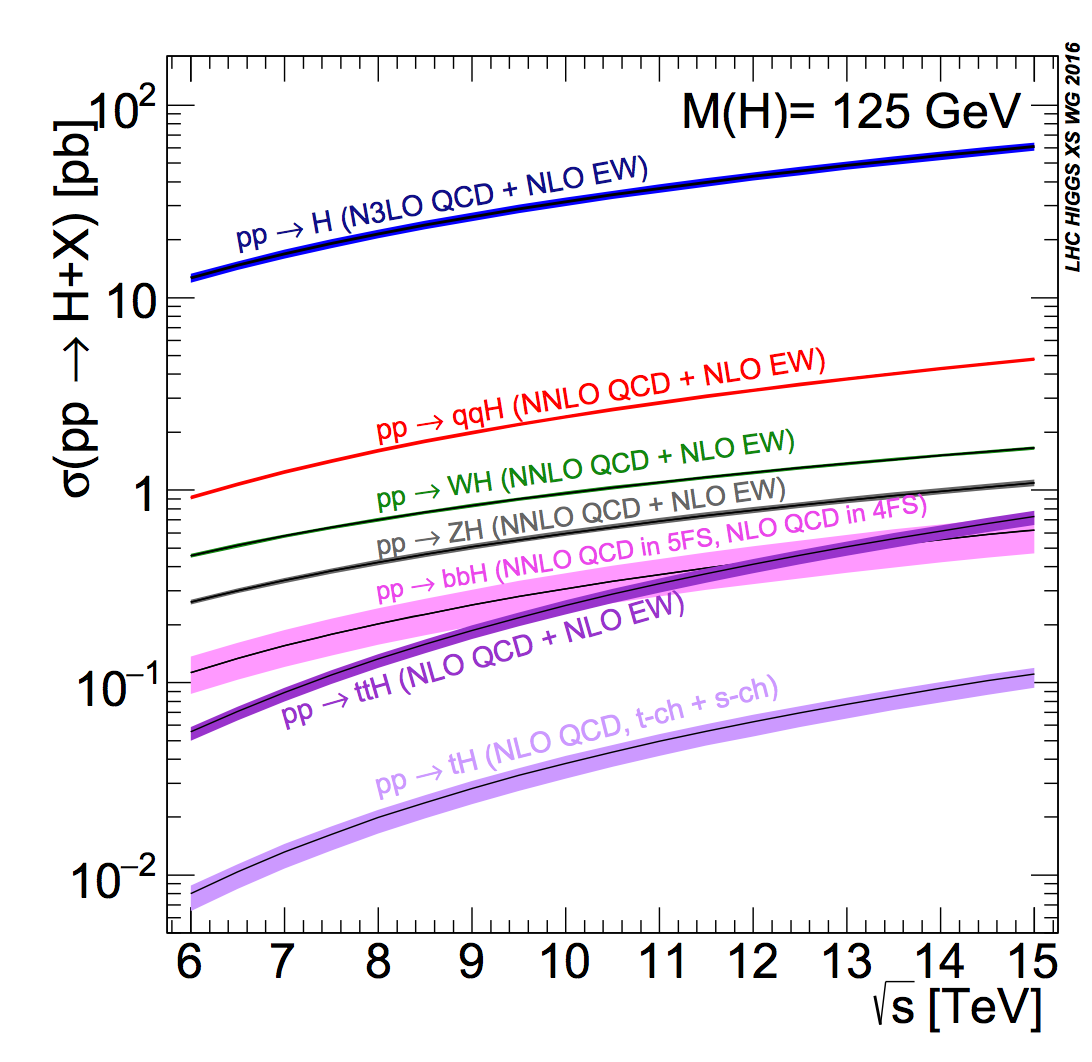
\includegraphics[width=1\linewidth]{/Introduction/Higgs/XsecHiggs}
	\end{minipage}
	\begin{minipage}[h]{0.54\textwidth}
		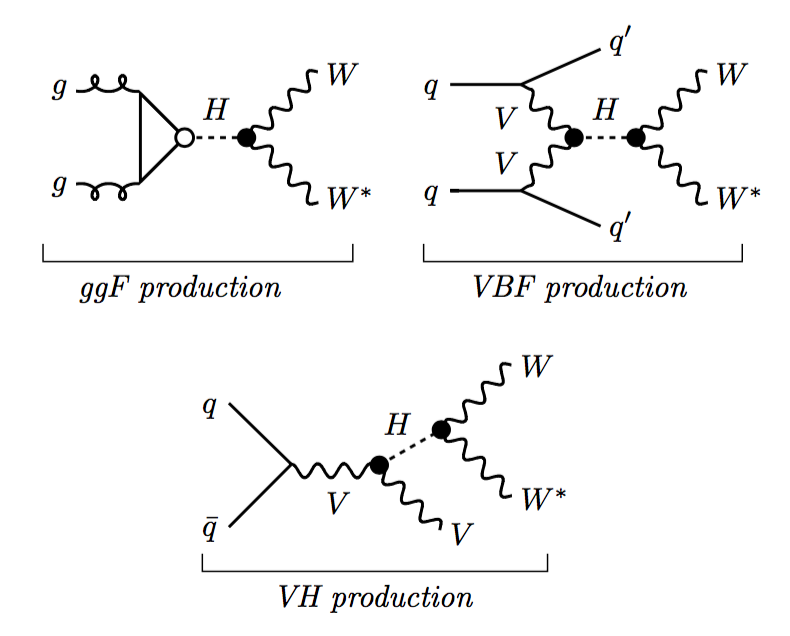
\includegraphics[width=1\linewidth]{/other/HIGGS_PRO}
	\end{minipage}
	\caption{Expected cross-sections of the productions of the Higgs bosons (left). The Feynman diagrams of the leading production modes of the Higgs boson which further decays to  $WW^{(*)}$ (right). Letter "V" represents a W or Z boson \cite{ATLAS:2014aga}.}
	\label{fig:Higgs_pro}
\end{figure}


\begin{figure}[!h]
	\graphicspath{ {./Figures/} }
	\centering
	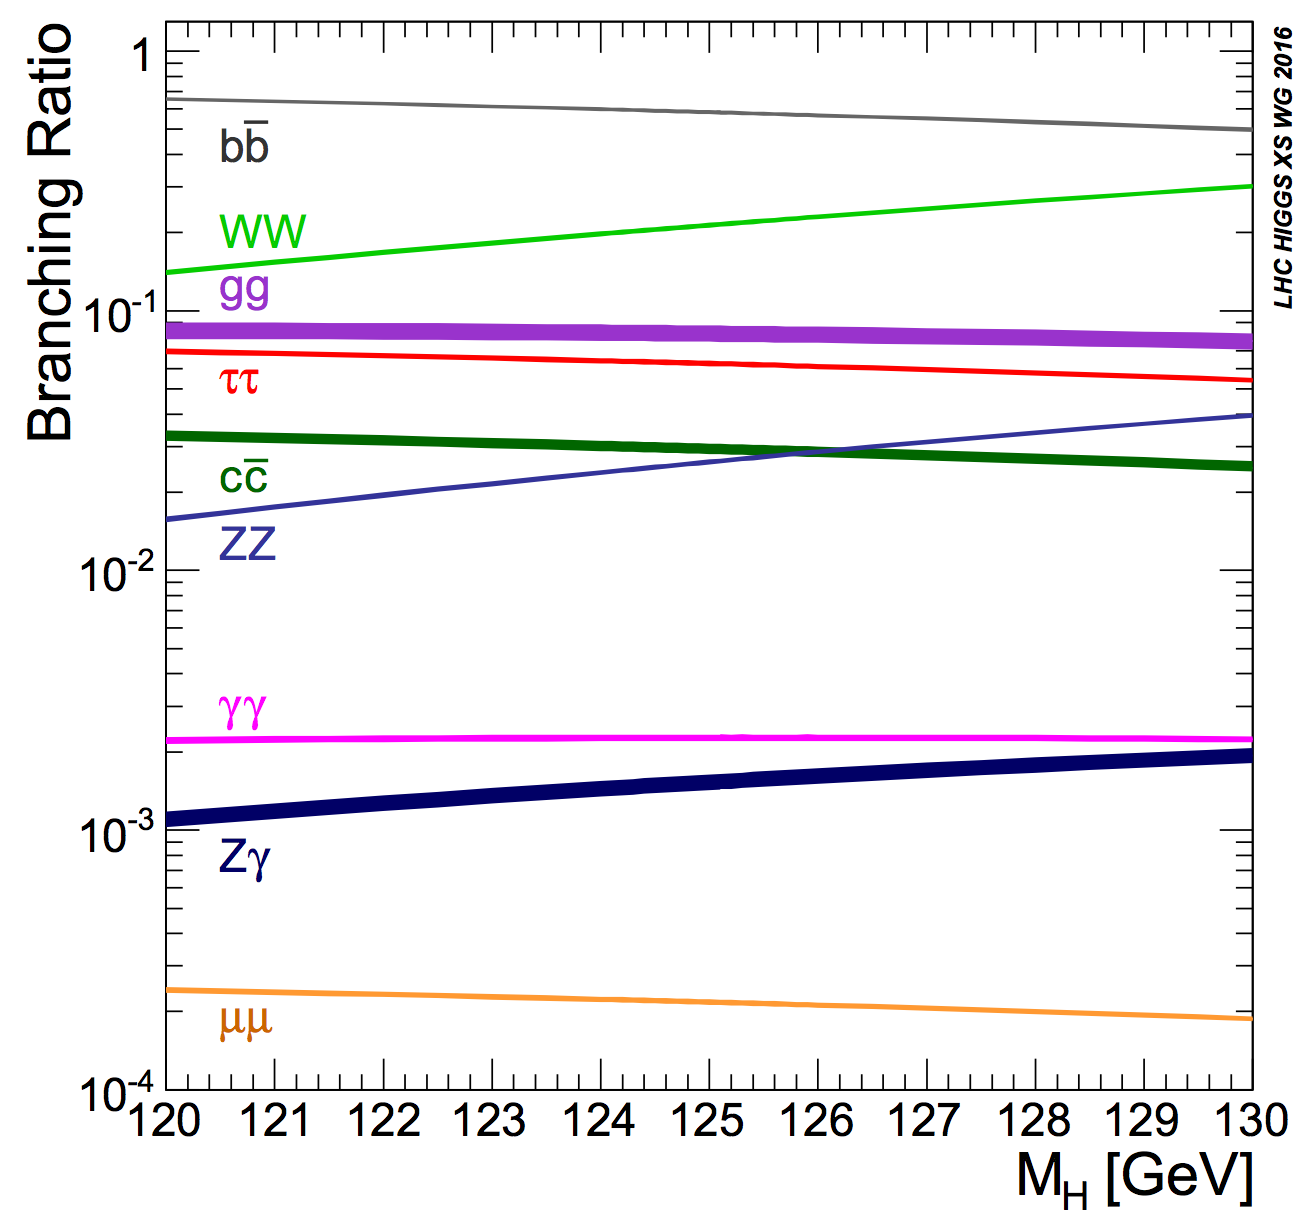
\includegraphics[width=0.5\linewidth]{/Introduction/Higgs/HiggsBR}
	\caption{Branching ratios of decays of Higgs bosons \cite{PDGReview}.}
	\label{fig:Higgs_decay}
\end{figure}





%==================== VBF HWW ====================%
